\documentclass[a4paper, USenglish, cleveref, autoref, thm-restate, final]{lipics-v2021}

%\nolinenumbers
\usepackage{hyperref}
\bibliographystyle{plainurl}

\title{Formally verifying a vertical cell decomposition algorithm}

\author{Yves Bertot}{Inria Center at Université Côte d'Azur, France}
       {yves.bertot@inria.fr}
       {https://orcid.org/0000-0001-5052-3019}{}

\author{Thomas Portet}{Inria Center at Université Côte d'Azur, France}
       {thomas.portet@inria.fr}
       {}{}


\authorrunning{Y. Bertot and T. Portet}

\Copyright{Yves Bertot and Thomas Portet}


\ccsdesc[300]{Theory of computation~Computational geometry}
\ccsdesc[500]{Theory of computation~Program verification}
\ccsdesc[500]{Theory of computation~Higher order logic}
\ccsdesc[500]{Theory of computation~Logic and verification}
\ccsdesc[500]{Theory of computation~Type theory}

\keywords{Formal Verification, Motion planning, algorithmic geometry}



%Editor-only macros:: begin (do not touch as author)%%%%%%%%%%%%%%%%%%%%%%%%%%%%%%%%%%
\EventEditors{John Q. Open and Joan R. Access}
\EventNoEds{2}
\EventLongTitle{42nd Conference on Very Important Topics (CVIT 2016)}
\EventShortTitle{CVIT 2016}
\EventAcronym{CVIT}
\EventYear{2016}
\EventDate{December 24--27, 2016}
\EventLocation{Little Whinging, United Kingdom}
\EventLogo{}
\SeriesVolume{42}
\ArticleNo{23}
%%%%%%%%%%%%%%%%%%%%%%%%%%%%%%%%%%%%%%%%%%%%%%%%%%%%%%

\begin{document}
\maketitle

\begin{abstract}
The broad context of this work is the application of formal methods to
geometry and robotics.
We describe an algorithm to decompose a working area
containing obstacles into a collection of safe cells and the formal
proof that this algorithm is correct.  We expect such an
algorithm will be useful to compute safe trajectories.

To our knowledge, this is one of the first formalization of such an
algorithm to decompose a working space into elementary cells that are
suitable for later applications, with the proof of correctness that
guarantees that large parts of the working space are safe.  Techniques
to perform this proof go from algebraic reasoning on coordinates and
determinants to sorting.  The main difficulty 
comes from the possible existence of degenerate cases, which are
treated in a principled way.
\end{abstract}

\section{Introduction}
The formal verification of algorithms is often presented as a solution
to avoid programming errors.  It is particularly suited to domains
where it is practical to give a mathematical description of the
problem and expected behaviors and where the cost of errors is
prohibitive.

In recent years, there has been much progress in the design and
acceptance of autonomous vehicles.
This domain seems suited for formal verification because it easy
rather practical to explain what situations constitute an error:
collisions between the controlled object and obstacles can be
described by some pair of set having a non-empty intersection.

One of the first case studies that comes to mind
is concerned with proving that a program producing trajectories for a
point in a 2-dimensional scene is safe.  We designed such a program.
Its first component is decomposing the scene into a collection of safe cells,
where each cell is a simple geometrical object.  Other components are
concerned with finding a path in a graph where the nodes are the safe
cells, connecting points inside or at the boundary of safe cells with
straight line segments, and then smoothing the angles of
that trajectory.  The first component is the
object studied in this paper, but the complete program and its
design choices are presented in \cite{bertot:hal-04312815}.
\begin{figure}
% trim left bottom right top
\begin{center}
\includegraphics[trim={0 24cm 0 2.0cm}, clip,scale=0.5]{main_program_steps.pdf}
\end{center}
\caption{The main steps of a trajectory computation: input, 
  vertical cells, piecewise straight trajectory, smooth trajectory}
\end{figure}

We chose to study an algorithm described in the book {\em Robot Motion
 Planning} by J.-C. Latombe under the name ``vertical cell
decomposition'' \cite{Latombe91} (pages 205--206).  In that book's
presentation, the obstacles are
described as polygons, but we simplify the problem by
considering only obstacles described using straight-line segments.
Our algorithm is thus an approximation, since the boundary of
any polygon can be viewed as a collection of straight edge segments.
To describe interiors of polygons as obstacles, we would need to add an
algorithm to compute the interior of polygons, which we believe to be
simple.

For now, we only consider the obstacles to be unsafe regions of the
working space, so we shall use the term {\em safe} for any point that
neither an event neither element of an obstacle.

Following this algorithm's description, each cell is either a
triangle or a trapezoid, with a bottom and a top side that are
straight lines, portions of the given obstacles, and lateral sides
that are vertical, as illustrated in Figure~\ref{fig:closed_cell}.
\begin{figure}[h]
\includegraphics[trim={0 19cm 0 4cm}, clip,scale=0.5]{one_closed_cell.pdf}
\caption{A closed cell: slanted dashed lines represent obstacles,
  vertical dotted lines are the lateral sides, solid black lines are
  the low and high sides of the cell.}
\label{fig:closed_cell}
\end{figure}

The vertical cell decomposition algorithm is a sweeping line
algorithm. It can be described
intuitively as the process of moving a line from left to right over
the scene, stopping each time an event is encountered.
Events occur when the extremities of obstacles are encountered.
Several obstacles may be involved in a single event: several
obstacles that were present on the left side the sweeping line may be
finishing at this event, and several obstacles may be starting at this
event.  The extra special case where an obstacle is vertical is not
treated by this algorithm.

When processing an event, the algorithm produces two kinds of cells.
Some of the new cells are {\em open}.  They are in a temporary state,
where only the left-hand side is known, actually this side is aligned
with the sweeping line.  The other new cells are {\em closed}.  These
cells are obtained by collecting all the existing open cells that are in contact
with the processed event and giving them a right side, again aligned with
the current location of the sweeping line.
Figure~\ref{fig:sweeping_steps} illustrates the progression of the
sweep line along several events.

\begin{figure}[h]
% trim left bottom right top
\begin{center}
\includegraphics[trim={0 24cm 0 2.0cm}, clip,scale=0.5]{sweeping_steps.pdf}
\end{center}
\caption{Sweeping through 4 events in a simple case.  For each event,
  the sweep line is shown as a vertical dash-dotted line,
  new open cells are shown with a striped pattern, new closed cells
  are shown with a tiled pattern.}
\label{fig:sweeping_steps}
\end{figure}

The lateral sides of each cell are vertical, because the sweeping line
is vertical.  Most of the points on these sides are safe, but
some are not,
because they are the location of an event, most often an extremity of an
obstacle.  The algorithm is designed in such a way that the unsafe
points on each lateral side are recorded in the data of each closed
cell (left points and right points in Figure~\ref{fig:closed_cell}).

For the use case that we have in mind, it is also important that cells
are non-empty.  To guarantee this property, we had to design specific
tests and corrective actions when two successive events are vertically
aligned.  So instead of processing events from left to right, which is
not precise enough, we process events in lexicographic order: from left to
right if the successive events have a different first coordinate, and
from bottom to top for events that have the same first coordinate.

The algorithm is described entirely using the functional programming
language of the calculus of inductive constructions, as implemented in
Rocq \cite{the_coq_development_team_2024_14542673}.  The input is given as a bounding box as specified by a bottom and
a top segments and a list of obstacles.
The output is a list of cells.  There are quite a few expected
properties for the inputs: the obstacles should all be entirely inside
the bounding box and no obstacle should be vertical.  In return, we
obtain a list of cells that satisfy a few properties.  In particular,
we define for each cell a safe part and an owned part.  For the safe part,
it is composed of two subparts: the interior of the cell (which is included in
the owned part) and the set of safe points on the lateral sides.  We
prove several inclusion and disjointedness properties for the obstacles, the
boundaries of cells and the interiors.  Altogether, we obtain a proof that
what we name the safe part of cells is indeed safe.

An extra property that we prove is that the center of each cell is an
element of the cell interior.

All these properties have been formally verified using the
Rocq prover and the {\sc Mathematical Components} library
\cite{assia_mahboubi_2022_7118596}.

There is an extra property for which the proof has not been done yet:
the union of all owned parts covers the inside of the bounding box.  Lacking
this property does not endanger the safety property, but a trivial algorithm
that returns an empty sequence of cells would satisfy the safety property.

The complete development of the algorithm and its proof is available
in the branch {\tt vertical-cell-paper} of a publicly
available repository
\begin{center}
\url{https://github.com/math-comp/trajectories/tree/vertical-cells-paper}.
\end{center}
This branch contains the snapshot that is described in this paper, but
the whole development is likely to evolve as more improvements are
added to the algorithm and the use case resting on it, as discussed in the
last part of this paper.

\section{The data components}
In this section, we describe the design choices for the various kinds
of data we manipulate in the algorithm.  The way we handle obstacles
deserves special attention.
\subsection{points and edges}

For the proofs, we assume that we work with a type {\tt R} of numbers
with the structure of a real field, as understood by the
{\sc Mathematical Components} library.  Among other operations, this
mathematical structure provides a boolean test for equality between
numbers and boolean test for comparison.  The library then provides a
lot of tools with their properties, like a boolean test for list
membership, sorting, etc.  In practice, this means that
the field of rational numbers is suitable for all computations
performed in this development.

Points are then described as pairs of numbers in {\tt R}, and edges
are described as pairs of points.  These data types inherit the
equality tests and the polymorphic functions for list membership of
the {\sc Mathematical Components} library can again be used for these
data types.  One peculiarity of our development
is that we chose to describe the edges as pairs of points with an extra
condition in our proofs: the first point has to have a first
coordinate that is strictly smaller than the first coordinate of the
second point.  This is an example of design where some data invariant
is hard-coded in the data structure.  As a result, the algorithm
cannot process vertical obstacles, because the data structure
representing the obstacles simply does not accept such cases.  In the
last part of the paper, we discuss ways to circumvent this limitation
concerning vertical edges.

The definition we use to introduce edges in our development is as
follows
\begin{verbatim}
Record edge := Bedge {left_pt : pt; right_pt : pt;
    _ : left_pt.x < right_pt.x}.
\end{verbatim}
This definition does not give a name to the condition that the left
point has a smaller first coordinate. Such a name is given later in
our development.

The most important basic block used in the algorithm is the
computation of whether a point {\tt p} is above or below an edge, or whether
it is aligned with the two extremities of the edge.  To compute this
condition, it is well known in computational geometry \cite{KnuthAxiomsHulls}
that the
following determinant can be used, where {\tt l} and {\tt r} are the
names for the left and right extremities of the edge:
\[\begin{array}{|ccc|}
1 & {\tt l}_x & {\tt l}_y\\
1 & {\tt r}_x & {\tt r}_y\\
1 & {\tt p}_x & {\tt p}_y\\
\end{array}\]
This is a determinant computation, and it is well known that this
determinant computes twice the {\em signed} area of the triangle {\tt
  lrp}.  The function {\tt area} computes this determinant.
Because it is a signed area, the value is positive if {\tt p}
is above and negative if {\tt p} is below.  We use the notations
{\tt \(p\) <{}<{}= \(g\)} and {\tt \(p\) <{}<{}< \(g\)} to express that a point
\(p\) is in the half-plane below an edge \(g\) or strictly below an
edge, respectively.

Because the algorithm uses a vertical sweeping line, our proofs
require that we check when a point is in the vertical cylinder
containing the edge.  This is simply done by comparing the point's
first coordinate with the first coordinates of the edge's extremities.
We write {\tt valid\_edge \(g\) \(p\)} to express that \(p\) is in
that cylinder.  We use the function {\tt point\_edge}, with the
notation {\tt p === g}, to express that
point {\tt p} is included in the obstacle {\tt g}.

When a point is valid for an edge, the vertical projection of that
point on that edge exists.  It is computed by a function called
{\tt vertical\_projection}.  Computing the vertical projection of a
point on an oblique edge requires that one computes a division. This
is the one place in the whole algorithm where division is used.
The function {\tt vertical\_projection} takes a point and an edge as
arguments and returns an {\tt option} type:
the projection is only computed if the point is in the vertical
cylinder given by the edge.  We prove a few properties of this
projection function: the point it returns is part of the edge on which
the projection happens, two points with the same second coordinate are
projected to the same point, and the input point and its projection
are vertically aligned.

We define a relation between edges, denoted {\tt <|} and called
{\tt edge\_below} which expresses
that the first edge is below the second one.  Edge \(g_1\) is below Edge
\(g_2\) if both extremities of \(g_1\) are in the half plane below
\(g_2\) or if both extremities of \(g_2\) are in the half plane above
\(g_1\).  During the operation of the algorithm, we use this relation
to sort edges going out of a given event.  For edges that all have the
same left extremity, the {\tt <|} relation is transitive, but in
general this relation is not transitive.
\subsection{The cells}
Each cell has a high edge, a low edge, a left side, and a right side.  For
the lateral sides, we record the ordered sequence of points that
correspond  to events in contact with this cell.  These points are
unsafe.  These two sequences of points are called the {\em left points} 
and {\em right points} of the cell (record projections
named {\tt left\_pts} and {\tt right\_pts} in the code).
These sequences are
ordered and contain no duplication, so that the open interval between two
points in a sequence is a door, a safe passage to another cell.

In the finished closed cells, the side point sequences are not empty,
as they always contain the projections of some event on the low and high
edge, which may be the same point.

As an intermediate data structure, we use cells where the
right-hand side is empty, called {\em open cells}, but in the code
it is never ambiguous whether some cell is open or closed.

The left points sequence of a cell is intended to contain
points that are vertically aligned, the first point is on the high edge
and the last point is on the low edge.  The same properties hold for the
right points.  We defined a predicate named
{\tt open\_cell\_side\_limit\_ok} to describe the properties of the
left points, and a predicate named {\tt closed\_cell\_side\_limit\_ok} to
describe the conjunction of the properties for the left and the right points.

We define the {\em left limit} of a cell to be the first coordinate of
the first left point, and similarly for the {\em right limit}.

The safe part of a cell is defined as the union of its strict interior
(points whose first coordinate is strictly between the left limit and the
right limit, strictly above the low edge, and strictly below the
high edge) and its doors (points on each of the sides that are
strictly above the low edge and strictly below the high edge and
different from the side points).  In what follows, the safe part of a cell
is described by a predicate named {\tt safe\_part}.


\section{The scan state}

The sweeping part of the algorithm is essentially a tail recursive
algorithm, consuming a sorted sequence of events and
maintaining a data structure which we call the {\tt scan\_state}.  This
structure contains a representation of the closed cells constructed so
far, a representation of all the open cells in contact with the
current position of the sweeping line, and some cached information:
the first coordinate of the last processed event, the high edge of the
last open cell.

The open cells are arranged in a vertically sorted sequence,
decomposed into three parts.  The middle part is a cell that is singled
out because it is the highest of the last created cells (in this
paper, we shall call this the {\em last open cell}).  The other two
parts are the prefix of the vertical sorted sequence before the last
open cell and the suffix of that sequence.

The closed cells are arranged in two parts, as the algorithm may need
to modify the last generated closed cell in some cases.

\section{The phases of the algorithm}
To organize the sweeping process, we work in two phases.
\begin{enumerate}
\item  We first
create a sorted sequence of events.
\item Processing this sequence of
  events actually implements the sweeping movement from left to right.
  For each event, it is removed from the sequence and the scan state
  is modified accordingly.
\end{enumerate}

An event is the pair of a point and a sequence of edges, with the
intended data-invariant
that all edges in the sequence have that point as their left
extremity.  In contrast with what was done for edges, we chose not
to encode this intended invariant in the data structure, but
events constructed in the algorithm are guaranteed to respect it.

To create the sequence of events,
we use a bespoke insertion-sort algorithm, where the insertion
procedure is designed to create new events only when no event with the
same point already exists in the sequence.  When adding edges to an
event, we do not produce a sorted sequence of edges.  Such a sorting
operation of the outgoing sequence of edges is performed later in the
algorithm.

When processing each event for the second phase,
four cases are treated differently:
\begin{itemize}
\item If the considered event is further right than the last processed event,
\item If the considered event is on the same vertical line, but above the
high edge of the last created open cell,
\item If the considered event is on the same vertical line, but below the
high edge of the last created open cell,
\item If the considered event is on the same vertical line and on the
  high edge of the last created open cell.
\end{itemize}

To obtain the initial scan state, we need to have already one closed
cell, which is only constructed after the first event is processed.
This assumes that the first event is not on the bounding box's left side.
This first closed cell has the left side of the bounding box as its left
side, and its right side contains exactly three points: the first
event, its projection on the high boundary of the bounding box, and its
projection on the low boundary of the bounding box.  The first
sequence of open cells is obtained by constructing new open cells
using the sorted sequence of outgoing edges from the first event.
When the first event has at least
one outgoing edge, the initial last open cell is a cell whose low edge
is the highest outgoing edge and whose high edge is the bounding box's
high boundary, with only two points in the left point sequence: the
projection of the event on the high boundary and the event itself (see Figure~\ref{figure:initial}).
When the first event has no outgoing edge (it is then handled as an
isolated obstacle), the initial last open cell
has the bounding box low boundary as low edge and the bounding box
high boundary as high edge, its sequence of left points contains the
event and the two projections on the boundaries.
\begin{figure}
\includegraphics[trim={0 23cm 0 0}, clip,scale=0.5]{initial_state.pdf}
\caption{\label{figure:initial}Two possible configurations for the initial scan state}
\end{figure}

\subsection{Work performed in the first case}
When the next event to be processed is not vertically aligned with the
previous one, we need to scan the current sequence of open cells to
know which of these cells will be affected by the current event.
These cells simply are the cells for which the current event is below
the high edge and above the low edge.  We call these cells the {\em
  contact cells}.  These cells are a sub-sequence
of the current sequence of open cells.  The function that computes
this sequence actually returns several meaningful pieces of data:
\begin{enumerate}
\item the prefix of unaffected cells,
\item the sequence of contact cells without the last one,
\item the last contact cell,
\item the suffix of unaffected cells
\item the low edge of the first contact cell,
\item the high edge of the last contact cell
\end{enumerate}
The function that computes this decomposition is called
{\tt open\_cells\_decomposition}.  It takes as input a point and a
sequence of cells.  We proved that under some assumptions, the
sequence of cells given as input is the concatenation of the prefix,
the contact cells, and the suffix, and that the two edges given as
output are indeed boundary edges of the first and last contact cells.

All contact cells are transformed into closed cells, by adding a
right-side.  When there is more than one contact cell, the first one
has as its low edge an edge that is not in contact with the current event
and as its high edge an edge whose right point is the current event.
Similarly, the last contact cell has as its high edge an edge that is not
in contact with the current event as its low edge an edge whose right
point is the current event.

When there is only one contact cell, this is because the processed
event is below that cell's high edge and above that cell's low edge.
The sequence of the right points for the new cell only contains three
points, the event and its projections to the cell's two edges.

All contact cells are removed from the list of open cells, but new
open cells, whose left side contains the currently processed event are
added in their place.  The new open cells are obtained by processing
recursively the sequence of outgoing edges, sorted with respect to the 
{\tt <|} relation (also known as {\tt edge\_below}).

\subsection{Work performed for the second case}
In the second case, we know that the last open cell is not among the
contact cells.  We call the function {\tt open\_cell\_decomposition},
but we only need to scan the suffix of the sequence of open cells (the
cells that are above the last open cell).  The rest of processing is
the same as in the first case, paying attention to the fact that the
prefix and the previous last open cell have to be included in the
resulting sequence of open cells.

\subsection{Work performed for the third case}
In the third case, the event is below the high edge of the last open
cell, and this event cannot be the right extremity of
an active edge, because there is no edge between the low and the high
edge of the last open cell.  For this reason, it is not necessary to
re-run the {\tt open\_cells\_decomposition} function, as it would
simply return the last open cell as the only contact cell.
Closing this contact cell to produce a new closed
cell is not suitable, because it would create an empty closed cell
(one where the lateral sides would be on the same vertical line).

No new closed cell is created, but the last closed cell needs to be
updated to the current event as an extra unsafe point on the right side.
This requirement explains why the scan state has a specific field for
the last closed cell.

New open cells need to be created.  If the current event has no
outgoing edges, then it is enough to update the last open cell by adding
the current event among its unsafe points on the left side.  If the
current event has outgoing edges, new open cells are created as in the
first two cases, but the sequence of unsafe points on the left of
the last open cell needs to be included in the sequence of left
points of the first newly created open cell.
\begin{figure}
\begin{center}
% trim left bottom right top
\includegraphics[trim={0 20cm 0 0}, clip,scale=0.5]{third_case.pdf}
\end{center}
\caption{Processing a degenerate case (third case):
  the processed event appears on
  the last open cell left boundary and on the last closed cell right
  boundary.  The unsafe points that were previously in the last open
  cell left point sequence need to be added to the first newly created
  open cell (here noted as {\sf new open cell \# 1}.
  }
\label{fig:third_case_degenerate}
\end{figure}

\subsection{Work performed for the fourth case}
In the fourth case, the processed event is on the high edge of the
last open cell.  We know that the last open cell will be the first of
contact cells, and we need to compute the other contact cells, by
calling {\tt open\_cells\_decomposition}, but this time with a sequence
of cells that starts with the last open cell.

When closing cells, the first contact cell does not need to be closed
and can simply discarded, because its left side is on same vertical line as
its right side, and all the unsafe points were already
taken into account by existing closed cells.

When creating new open cells, special attention is required for the
case where the event has no outgoing edges.  In this case, the last
open cell needs to be replaced with an open cell that has as low edge
the same low edge as the the last open cell, as high edge the high
edge of the last contact cell
(as computed by {\tt open\_cells\_decomposition}) and as sequence of
last points the sequence of left points from the last open cell where
the projection on the high edge has been added.

\subsection{Specifying the safety property}
The safety property will
be expressed in the following manner: any point in the safe part of a
closed cell is distinct from the obstacles and the events given as
input.  We already defined the safe part of closed cells in the
section about cells.

In a similar manner, we can describe unsafe locations as the union
of points lying on an obstacle, as described by the function
{\tt point\_on\_edge} and the set of orphaned events.  In practice,
we can define a predicate {\tt unsafe} that takes as input a sequence
of events and a point to describe this space.

We prove that the intersection between unsafe locations and the union
of all safe parts of the resulting closed cells is empty.

However, we have to be careful because this proof is done under a
collection of assumptions.
\begin{itemize}
\item The type of numbers provided to describe the point coordinates,
  the edges, alignment of points, and so on, with its operation and
  comparison predicates forms an ordered field structure.  It means that the
  algorithm only uses addition, multiplication, and their inverses.
\item The only allowed intersections between obstacles are at their
  extremities.  Removing this constraint is planned as future work.
\item The sequence of obstacles does not contain any duplications.
\item There is a bounding box, given by a bottom and a top edge and two
  lateral sides, which contains all events.  In particular, this bounding box
  has distinct lateral sides and bottom and top edges (the bottom edge being
  below the top edge).
\end{itemize}
When propagating this specification to the two phases, it turns out we
need the following specification for the sorting phase.
\begin{enumerate}
\item The union of all outgoing edges of all events in the sorted
  sequence of events contains the initial obstacles.
\item For every event, all outgoing edges have the same left
  extremity, located at this event.
\item For every event, the sequence of outgoing edges has no duplicates.
\item The sequence of events is strictly sorted lexicographically.
\item No event in the sequence appears in the middle of one of the
  obstacles.
\item The right extremity of every outgoing edge is also located at an
  event existing in the sequence of events.
\item There are no intersections between pairs of edges except at their
  extremities.
\item All events are inside the bounding box.
\end{enumerate}
The second part of the program, which processes the sequence of events
does not make the assumption that events are always edge extremities.
When specifying the safety
property for the results of the algorithm, we simply need to make sure
that these orphaned events are excluded from the safe subset of the
configuration space.

A property that does not appear immediately as a safety property is
that the middle of every cell is strictly included in the cell.  This
property is useful for users of this algorithm who wish to use a cell
as a maneuvering space to move from one door of the cell to another door of
the same cell, when both doors are on the same side.  This property is
the main reason for having a specific treatment for degenerate cases.
This specific treatment actually guarantees that every closed cell has
a left-hand side that is further to the left than the
right-hand side.

To make sure that every cell contains at least a safe point, we
actually need the property that every event has a list of outgoing
edges without duplication.  Our code to generate the sequence of
events does not include steps to guarantee this, but we guarantee
that it operates correctly if the input
list of obstacles has no duplicates.

Finally, the statement we prove for the second phase is the following one,
as written in the input language of the Rocq prover (by taste, we prefer
to avoid special characters).  In this statement, the function
{\tt complete\_process} represents the algorithm that processes the sequence of
events: it combines together the operation of constructing the first cells
from the first event, and processing the last open cell to create the rightmost
closed cell.  The function {\tt events\_to\_edges} collects all the edges
from a sequence of events.
\begin{verbatim}
Lemma second_phase_safety (bottom top : edge) (evs : seq event) :
  well_formed_bounding_box bottom top ->
  {in bottom :: top ::
       events_to_edges evs &, forall e1 e2, inter_at_ext e1 e2} ->
  all (inside_box bottom top) [seq point e | e <- evs] ->
  sorted (@lexPtEv _) evs ->
  {in evs, forall ev, out_left_event ev} ->
  close_edges_from_events evs ->
  {in events_to_edges evs & evs, forall g e, non_inner g (point e)} ->
  {in evs, forall e, uniq (outgoing e)} ->
  {in complete_process bottom top evs, forall c,
    strict_inside_closed (cell_center c) c /\
    closed_cell_side_limit_ok c /\
    forall p, cell_safe_part c p -> ~ unsafe evs p}.
\end{verbatim}
This statement has 8 prerequisites, mostly expressed as properties of the
sequence of events.  Among notations, {\tt \{in F, forall x, \dots\}}
represents a universal quantification over all elements satisfying {\tt
  F}, {\tt \{in F \& G, forall x y, \dots\}} represents two
quantifications over elements in {\tt F} (for {\tt x}) and {\tt G}
(for {\tt y}), {\tt \{in F \&, forall x y, \dots\}} represents two
quantifications both ranging over elements in {\tt F}.

A more compact statement can be used if we consider the combination of the
two phases, because the first phase guarantees the prerequisites on the
sequence of events.  The combination of the two phases is called
{\tt edges\_to\_cells} in this statement.
While the concision of this statement is pleasant, it
misses some of the power of the second phase.
\begin{verbatim}
Lemma two_phase_safety bottom top (edges : seq edge) :
  well_formed_bounding_box bottom top -> uniq edges ->
  {in bottom :: top :: edges &, forall e1 e2, inter_at_ext e1 e2} ->
  {in edges, forall g p, p === g -> inside_box bottom top p} ->
  {in edges_to_cells bottom top edges, forall c,
    strict_inside_closed (cell_center c) c /\
    closed_cell_side_limit_ok c /\
    forall p, cell_safe_part c p -> {in edges, forall g, ~ p === g}}.
\end{verbatim}
This lemma only has 4 prerequisites: the bounding box given by the
bottom and top edges must define a workable area of the plane, the sequence
of input edges must have no duplication, considered edges may only
meet at endpoints, and all edges must be inside the bounding box.  With these
four prerequisites, the algorithms of the first phase are able to produce
a sequence of events satisfying the eight prerequisites of the second phase.

As a result, the algorithm produces a sequence of cells that satisfy three
properties: each contains at least one point, they are well formed (the 
sequence of points on the side are vertical and ordered, the extremities of
these sequences are on the low and high edges of the cell) and the safe
part has an empty intersection with the union of the obstacles.

\section{Proving the safety property}
\subsection{Mirroring contexts}
The infrastructure of definitions provided by the {\sc Mathematical
Components} library is not fully compatible with the extraction
process provided by the Rocq prover \cite{letouzey:hal-00150914}.
To obtain code that is amenable for extraction, we write a
first file called {\tt generic\_trajectories}, that does not rely on
any of the mathematical structures of the library, but is
parameterized by a given type supposed to represent numbers, with 4
operations (addition, subtraction, multiplication, division) and two
comparisons.  Also, this algorithm relies on a degraded type of edges,
where the condition that the first point is on the left of the second
point is absent from the data-structure.

The generic algorithm is used in all the proof files.  In each of
these proof files, we actually instantiate the type of numbers with
a mathematical structure from the {\sc Mathematical Components} library.
Following the library's idiom, we do not choose a specific field structure,
we assume we are using one that exists.  So, the proofs we make are assuming
that the user of the code also respects that part of the specification and
actually instantiates the software with a number structure that respects the
properties specified by the real field structure.

We do provide a running implementation by instantiating the
type of numbers with rational numbers, implemented as a pair of a numerator
(an integer) and a denominator (a positive integer).

Every function imported from {\tt generic\_trajectories} is a function
with at least 7 arguments.  To make the whole setup comfortable, a
header of notation definition is provided to instantiate the function
to the type and operations provided by the field structure.  This header of
notations needs to be repeated in each working file, because the field
structure named {\tt R} in each file is conceptually a different structure
for each file.   However, theorems proved in one file can be reused in another
simply because they are generalized at the end of each section and can be
re-instantiated at each usage.

\subsection{Main organization of the proof}
\label{sec:invariant_levels}
The first part of the algorithm consists in preparing the list of
events so that processing these events in the order given by the list
simulates the intuitive behavior of moving a vertical line
from the left-hand side of the box to the right-hand
side.  Proving that this sorting algorithm guarantees the properties
required by Lemma~{\tt second\_phase\_safety} is comparatively easy.
However, this lemma only expresses safety with respect to the obstacles and
points found in the list of events.  Therefore, an extra property that is
important is that the edges present in the resulting
list of events are the input edges.

We will now concentrate on the second phase.
We established six levels of invariants:
\begin{enumerate}
\item In the first level, we state properties that concern the
sequence of open cells and the relations between their edges and the remaining
events.
\item In the second level, we add properties that fall in three categories:
  \begin{enumerate}
    \item The cache consistency properties of
  the scan state: the scan state contains a last open cell, a last high edge,
  and a last {\tt x} coordinate.  It is assumed that the last high edge
  is the high edge of the last open cell, and that the last {\tt x} coordinate
  is the left limit of the last open cell.
\item The expected properties of the remaining sequence of events: these
  events are ordered lexicographically, all the right extremities of their
  edges are also covered by events in the sequence, the field {\tt outgoing}
  of each event is a list that only contains edges whose left-hand extremity
  is on this event, and this list has no duplicates.
\item There is no intersection between the high edges of all open cells
  and the outgoing edges of events in the sequence of events.
\item The bottom left corner of the last open cell is lexicographically
  smaller than any event in the sequence.
\item If the sequence of events is not empty, the next event is
  lexicographically larger than the left extremity of all edges of
  open cells, and lexicographically smaller than the right extremity.
\end{enumerate}
\item In the third level, we add properties that are specific to the
  last created open cell,
\item In the fourth level, we add mainly the properties that concern
  the closed cells that were built so far and their interactions with
  the current open cells.  The main purpose of the properties
  available in this invariant is to contribute to the proof that
  all closed cells are disjoint and non-empty.
\item In the fifth level, we add mainly the properties that concern
  edges that were outgoing from events that have already been processed.
  In particular, we concentrate on properties that are useful to show that
  all these edges are covered by the top side of existing closed cells and
  existing open cells.
\item In the sixth level, we add mainly the properties that concern
  the points recorded in cell sides.  The aim is to show that cell
  sides enumerate the points that are unsafe on the lateral
  sides of cells.
\end{enumerate}

In the end, the safety property for the space inside a given cell is
guaranteed by the main argument that if edges are covered by the high
edges of all closed cells, and all closed cells are disjoint, then
edges cannot appear in the interior of a given cell.

When addressing a complex algorithm like the one presented here, it is
possible to develop a simpler proof of the main result, obtained under
stronger assumptions concerning the inputs.  We performed such a
simpler proof, which expresses how the algorithm works in cases where
no events are vertically aligned.  This proof relies on simpler
invariants and leaves some branches of the code unverified.  Still it
was useful to us a a means to explore the structure of the more
complete proof.  In our formal development, the simpler proof is found in files
{\tt general\_position.v} and {\tt safe\_cells.v}.
In this paper, we concentrate on the second, more complete proof.  The
main lemma for that simple proof is named {\tt
  start\_yields\_safe\_cells} in file {\tt safe\_cells.v}.

\subsection{The area function and the {\tt edge\_below} relation}
The signed area function is instrumental to detect when a point is above or
below an edge.  More precisely, it makes it possible to detect when a
point is above the straight line that carries the obstacle.

This area function is given by a determinant formula that we learned
from Knuth \cite{KnuthAxiomsHulls}.
It is quite important that this is only computed using a
determinant, as it only needs ring operations (no division), without
ever mentioning the projection of the given point on the given
straight line.

For proofs, however, it is useful to have an alternative point of view,
where one expresses the property of being above using a comparison of
the second coordinates of the given point with the projected point on
the given line.

The edge comparison relation, called {\tt edge\_below} and
noted {\tt <|} is directly related with the area
function.  To detect whether an edge is below another, we simply
verify whether the two extremities of one are in the same half-plane
with respect to the other.

It turns out that this relation is reflexive, not transitive, and not
antisymmetric.  We spent quite some time trying to show that it is transitive
on some well-chosen subsets, but this turned out to be unproductive.  For
this reason, it is not very useful (although it is true) to show that the
sequence of high edges of all open cells is sorted for the {\tt edge\_below}
relation.  We
finally chose to express that this sequence of edges
satisfies a stronger invariant: an edge \(g_1\) that appears before an edge
\(g_2\) in this sequence is below.

All open cells intersect with the sweeping vertical line.  As a
consequence, it is useful to have a collection of lemmas establishing
correspondences between edges below one another and the second coordinate
of the projection of a point on these edges.  This is quite natural to
express but one must be careful to only consider points that are in
the intersection of vertical cylinders above the two edges.  The lemmas
have names like {\tt order\_edges\_viz\_point} or {\tt under\_pvert\_y},
sometimes with a {\tt strict} qualifier added.

\subsection{Building up invariants}
\subsection{The key property of disjoint cells}
In the end, each closed cell has four boundaries: two vertical ones, a
low boundary (a fragment of an obstacle that is not vertical) and a
high boundary (again, not vertical).  We define three zones:
\begin{itemize}
\item inside the union of the cell and its boundaries,
\item in the interior of the cell (in the cell, on not on the boundaries),
\item inside the cell and its
 boundaries, but neither on the bottom boundary nor on the left
 boundary.  In the rest of the paper, we say a point that satisfies
 this property with respect to a cell is {\em owned by the cell} (in the
 own part of the cell).
\end{itemize}
The main key property that we want to guarantee is that every point
strictly inside a cell does not belong to any obstacle.  To establish
this, we decompose the problem into three parts: first, we show
that points can only be owned by one cell.
Then, we prove that every obstacle is included in the union of high boundaries of
all cells.  As an immediate consequence, the interior of a cell doesn't intersect
with the obstacles.  The third property focuses only on the
lateral sides of cells.

To prove that closed cells are disjoint, we need to prove that new
cells added at each iteration are disjoint with the existing ones.
The new closed cells actually come from
existing open cells.  Thus, we need to prove that
closed cells are kept disjoint from open cells, and in turn, we need to
show that open cells are disjoint.

The position of the sweeping line plays an important role when proving
that existing closed cells and open cells are disjoint.  At any
iteration, the newly created open cells have their left side on the
sweeping line.  On the other hand, newly closed cells have their right
side on the sweeping line.  Moreover, since the sweeping line is moving
from left to right, all previously existing closed cells have their
right side on the left of the sweeping line.  This guarantees that newly
created open cells are disjoint from all closed cells, whether new or
previously existing.

In the degenerate case where two successive events are vertically
aligned and the second event lies below the high edge of the last
closed cell created when processing the first event, this last closed
cell is modified and the new modified cell becomes the last closed
cell after processing the second event.  We need to guarantee that
the modification does not interfere with the disjointedness property with
respect to the other cells.  We use the fact that
points attached to the last closed are the same before and after the
modification (which consists only in adding the second event to the
sequence of right points in the cell, in second position).
\subsection{Obstacle covering}
The obstacles whose left extremity is at an event that has already been
processed are covered by the high boundaries of existing closed cells and
open cells.

An obstacle (an edge) \(g\) is covered by the sequence of closed cells if
there exists a sequence of cells \(s\) included in the closed cells
with the following properties:
\begin{itemize}
\item all cells in \(s\) have \(g\) as their high edge,
\item in \(s\), each cell's right limit is the next cell's left limit,
\item the first cell's left limit is the first coordinate of the obstacle's
  left extremity.
\item the last cell's right limit is the first coordinate of the obstacle's
  right extremity.
\end{itemize}
Some obstacles are only partially covered by the closed cells, but in that
case their right part is covered by an open cell.  In that case, there
is a sequence \(s\) included in the closed cells
and an open cell \(c_o\) such that:
\begin{itemize}
\item all cells in \(s \cup \{c_o\}\) have \(g\) as their high edge,
\item for the sequence \(s\) followed by \(c_o\) each cell's right limit
  the next cell's left limit.
\item the first cell's left limit is the first coordinate of the obstacle's
  left extremity.
\end{itemize}

When an event is processed, the cell decomposition algorithm computes
a sequence contact cell together with a last contact cell.  Its high edge
is the same obstacle as the high edge of the future last open cell.  If we
are in general position (the current event is not vertically aligned
with the previous one), this high
edge was covered by the combination of a sequence of closed cells and
an open cell (the last contact cell) before this iteration,
and after this iteration, the coverage is ensured by a new sequence
of closed cells which is the same as previously with a new closed cell added,
obtained by closing the last open cell, and the last of newly created open
cells covers the rest of that obstacle.

For the high edges of all the other contact cells, they are
necessarily ending in the current event.  So, these obstacles move from
the category of obstacles that are partially covered by open cells to
the category of obstacles that are completely covered by closed cells.

If we are in the degenerate position where the current event is
vertically aligned with the previous event and below the high edge of the
last closed cell, then the sequence of closed cells that participate
in covering this edge keeps the same number of elements: the previous last
closed cell is removed and replaced by the modified closed cell
where the event is added among its right points.  The portion of the
obstacle that is covered by the previous last closed cell and the
modified cell is the same.  Concerning coverage by an open cell, the
new last open cell has the same high edge as the previous one, and
they have the same left side, because the two events that created
these open cells are vertically aligned.
\subsection{Safety for points strictly inside cells}
In the end, there are no more events left to process, so that all
obstacles are covered by closed cells.  
We can guarantee that points strictly inside these closed cells are not
on obstacles by combining the edge covering property and the
disjointedness property.  If we name \(c_1\) a closed cell and \(p\) an
point inside that cell, then \(p\) cannot be on the high edge of
\(c_1\) by definition of ``strictly inside''.  If \(p\) is on an
obstacle, this obstacle is covered by cells, so that there must be a
cell \(c_2\) such that \(c_2\) contains \(p\) and \(p\) is on the high
edge of \(c_2\).  Because \(p\) is not on the high edge of \(c_1\),
\(c_1\) and \(c_2\) must be distinct, but by the definition of
owned points, \(p\) must be attached to both \(c_1\) and \(c_2\).
\subsection{Safety for points on the lateral boundaries}
For points on the lateral sides, we first concentrate on the left side.
When an event is processed, closed cells have a left limit that is
strictly lower than the event's first coordinate, so that this event cannot appear
in the safe left side of a closed cell.  For the open cells, we show
that all the cells that are not in contact have their left side preserved.
So in the end, we only need to show that the created open cells do contain
the current event in the left points, so that this event is not considered
safe by these cells.

In degenerate situations, it happens that some newly created
open cell has a left side that overlaps with a previously
existing last open cell.  In that case, we do prove that the existing
unsafe points from the previously existing cell are inherited by the newly
created open cell.  This situation is depicted in
Figure~\ref{fig:third_case_degenerate} (a few pages before).

Proving that all cells have a safe right side follows a similar track.
Apart from the last closed cell, we know that no closed cell is in contact
with the currently processed event, either because the closed cell is
further to the left of the sweeping line, or because the closed cell has
a top-left corner that is strictly lower than the current event.  The
latter property is part of the invariant at sixth level, as described
in Section~\ref{sec:invariant_levels}.

When creating new closed cells (in the first two cases and the fourth one),
the proof proceeds by checking that the sequence of the right points
for all newly created cells contains the currently processed event.
In the fourth case, it happens that the cell obtained by closing the
first contact cell is discarded (because its left side and right side
stand on the same first coordinate).  But we show that all points
that would have been on its right side are already covered by existing closed
cells.

In the third case, where the last closed cell is simply obtained by
taking the previous last closed cell and adding the currently processed event
in the sequence of right points, it is easy to show that all points
that were already marked as unsafe are still marked as unsafe, together with
the currently processed event.

In the fourth case, the currently processed event is not added to the
sequence of right points of the previous last closed cell, because it
was already present in that sequence: this event is on the high edge of
the cell, so it is already equal to the projection of the previous event
on that edge (because the processed event and the previous event are on
the same vertical).

\begin{figure}
\begin{center}
% trim left bottom right top
\includegraphics[trim={0 23.2cm 0 2cm}, clip,scale=0.5]{sides_4th_degenerate.pdf}
\end{center}
\caption{Processing a degenerate case (fourth case):
  in the figure on the left, the situation is not degenerate, the
   processed event is the right extremity
  of an edge, and further right than the top-right corner of the last
  closed cell (square tile pattern).
  A   thin closed cell is created below and to the left of the processed
  event (dotted pattern) and another closed cell
  is created above that edge (zigzag pattern).  If the processed event
  is the top-right corner of the last closed cell, as in the figure on
  the left, the first closed
  cell vanishes.  The algorithm is designed in such a manner that the
  unsafe points are recorded in the right sides of the various
  preserved closed cell, and also in the left side of the newly
  created open cell.
  }
\label{fig:third_case_degenerate}
\end{figure}
% 30.061 53.620 49.600 55.965
% 51.153 39.
% 133.639 39.166
\section{Conclusion}
In our development, the code of the algorithms is in a
file named {\tt generic\_trajectories.v}.  This file does not only contain
the vertical cell decomposition algorithm, but also some more code to compute
trajectories based on the cells that are obtained, with the aim of building
a piece of software used in outreach activities.

The part that is concerned with only computing the vertical cell decomposition
culminates with Function {\tt edges\_to\_cells}, defined at line 507.
This prefix actually contains 381 lines of algorithm description, the
rest being blank or comment lines.

The proofs span 12 files, visible in the supplementary material \cite{suppl_material}.
There are almost 15000 lines of proof.  The supplementary material also
contains a demonstration tool, where users can give obstacles one by one
and see the decomposition in vertical cells being computed after each
interaction.  The demonstration tool also computes trajectories, but the
algorithm to compute these trajectories is outside the scope of this paper.

It is often advocated that one should have a complete proof
infrastructure before starting a formal proof.  This is not the
approach that was followed here.  We took an algorithm from a book
description, a junior member of the team implemented it in the
functional programming language of the calculus of inductive
constructions, and we started to prove simple invariants about this
algorithm, as this was also understood as an opportunity for the junior
member of the development team to train on formal verification.

During the same period, we had discussions and reflections on the way to
state and verify a reasonable safety specification.  Thus, we came up with the
crucial invariant that two distinct cells had disjoint owned parts.  We then
started proving that invariant under the strong assumption that there
were no degenerate cases (events are never vertically aligned).

This proof was done in a progressive manner: every time we came
across the need for a property that seemed reasonable, we would add it to
a large collection of invariants as an assumption and finish the needing proof.
Later, we would attempt to prove all the invariants, thus requiring possibly
more.  This trial-and-error approach may seem clumsy, but it also illustrates
that the formal verification process can help the proof designers organize
their thoughts.  The main remnant of that period is Section~{\tt step} in
file {\tt cells\_alg.v}.

When the proof under the strong assumption was complete, we wrapped up the
results in files {\tt general\_position.v} and {\tt safe\_cells.v}.
We started to prove the more general statement, accepting events that
would be vertically
aligned.  While performing that proof, we discovered that each degenerate
case required lengthy proofs, which we chose to store in separate files:
{\tt initial\_cell.v}, {\tt simple\_step.v},
{\tt first\_degenerate\_position.v}, and
{\tt second\_degenerate\_position.v}.  In the end, the proof of the main
safety statement is in file {\tt step\_correct.v}.

In the end, there were so many invariant properties that we decided to group
them into packages, which are the several levels of invariants presented
in this paper.  In this process, some redundancies between invariants were
detected and removed (often relying on a small lemma to show that a redundant
lemma is an easy consequence of other invariants).  We do not use the same
packages for the proof in the general position (with no vertical alignment
between events) and for the strong proof.

The resulting proof is still very large and difficult to share between several
developers.  We believe that the whole formal document should probably be
re-factored to improve its readability and long-term maintainability, but it
has reached a state that is ready for external usage: the code can be executed
and its specification is concise enough to make further usage in larger
applications feasible.

\subsection{A basis for trajectory computation}
As a way to assess usability, we integrated this program into a larger
application that produces trajectories without intersections with
the obstacles between points inside the bounding
box, when possible.  To work properly, this larger application relies
on a few more properties that we have not included in our specification yet.
Here are two examples of such properties:
\begin{itemize}
\item The set of created cells should cover the whole interior of the
  bounding box
\item When there exists a safe passage between two adjacent cells, these
  cells actually have a door in common.
\end{itemize}
According to our tests, these properties hold for our algorithm, but
they have not been proved formally.  If these properties were not satisfied,
the program would not compute trajectories between some points that can
actually be connected by such a trajectory.

\subsection{Related and Future work}
The literature of formal verification has few examples of verification for
algorithms coming from computational geometry.  Pichardie and Bertot
\cite{pichardie:hal-01702679} published
formally verified proofs of convex hull algorithms in two dimensions.  They
describe the determinant that can be used to know whether a point is on the
left or the right of an oriented segment.  We re-use that determinant in our
work, to detect when a point is above or below an obstacle, because our
obstacles can naturally be viewed as oriented segments (from left to right).
Convex hulls, have been studied formally again in the work of Brun, Dufourd,
and Magaud \cite{brun:hal-00955400}, but this time the aim was to illustrate
the use of a general data structure to describe sub-divisions of the plane,
called hypermaps.  Our work makes no use of hypermaps.  Another formally
verified work using convex hulls is the work of Immler on
zonotopes \cite{ImmlerZonotopes15}.

Geometry and convex hulls also play a significant role in two recent
formalization efforts focused on mathematical riddles.  F.~Maric
developed a formal proof of a conjecture of Erdös, that every set of
points \(2 ^ {m - 2} +1\), with \(m \geq 3\) contains a convex polygon
with \(m\) sides, but just for the value \(m = 6\).
\cite{Maric2019} and B. Subercazeaux et al. developed a similar proof
for the solution of a similar problem, where the convex polygon has to
be empty, again for the value \(m = 6\)
\cite{subercaseaux_et_al:LIPIcs.ITP.2024.35}.  Both developments are
characteristic in the use human expertise to reduce the problem to a
discretized problem that is then solved using an automatic SAT solver,
thus relying on proofs that cannot be check by the human eye.  The
reduction is formally verified using a interactive theorem prover, in
the former case Isabelle/HOL and in the latter case Lean.

Motion planning is an envisioned application domain for the work presented
here.  Motion planning has also been studied formally, by Rizaldi and 
their co-authors \cite{Rizaldietal18}.  This experiment is quite remote from
ours, as they rely on an interaction between the proof assistant {\sc Isabelle}
and another symbolic engine to obtain trajectories paired with a proof.  The
work described in this article is less complete since we do not show how
to compute trajectories, but it also places itself at a different level of
interaction: we provide a correctness proof for an algorithm that can run
independently from the proof assistant that was used to prove its correctness.
Anand and Knepper \cite{AnandRoscoq15} also concentrate on robot
trajectories, but they do so for a single maneuver, checking that all
numeric computations combine to guarantee that the robot will reach the
prescribed destination, while we are interested in the preliminary step
of decomposing the configuration space into cells where movement will be safe).

As future work, we wish to work in three directions.  The first direction
is to refine the algorithm to make it more efficient: for instance,
each cell should contain a reference to its neighbors, so that computing
the neighbors can be done in constant time, instead of the current situation
where all existing cells must be visited to find the ones that have a door
in common.  The second direction is to make the algorithm stronger, 
by accepting vertical obstacles and by accepting obstacles that cross.
The third direction is to work on trajectory computation, either by proving
formally the correctness of a prototype that we already designed using
Bezier curves, or by
designing a variety of planning algorithms relying on different kinds
of curves.
\bibliography{main}


\end{document}

